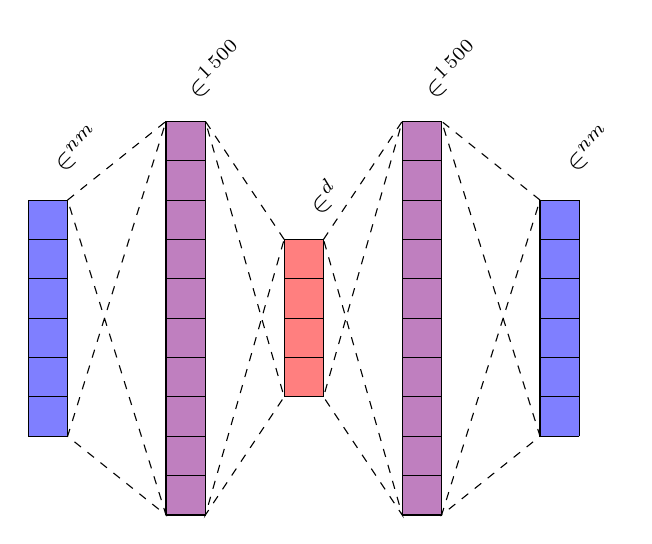
\begin{tikzpicture}[scale=0.5]
%\draw[thin, opacity=0.5] (-7.5,-6.5) grid (7.5,6.5);

%%% vecteurs

% input
\draw[fill=blue, fill opacity=0.5] (-7,-3) -- (-7,3) -- (-6,3)  -- (-6,-3) -- (-7,-3);
\draw (-7, 2) -- (-6, 2);
\draw (-7, 1) -- (-6, 1);
\draw (-7, 0) -- (-6, 0);
\draw (-7, -1) -- (-6, -1);
\draw (-7, -2) -- (-6, -2);

% hidden 1
\draw[fill=violet, fill opacity=0.5] (-3.5,-5) -- (-2.5,-5) -- (-2.5,5)  -- (-3.5,5) -- (-3.5,-5);
\draw (-3.5, 4) -- (-2.5, 4);
\draw (-3.5, 3) -- (-2.5, 3);
\draw (-3.5, 2) -- (-2.5, 2);
\draw (-3.5, 1) -- (-2.5, 1);
\draw (-3.5, 0) -- (-2.5, 0);
\draw (-3.5, -1) -- (-2.5, -1);
\draw (-3.5, -2) -- (-2.5, -2);
\draw (-3.5, -3) -- (-2.5, -3);
\draw (-3.5, -4) -- (-2.5, -4);

% latent
\draw[fill=red, fill opacity=0.5] (-0.5,-2) -- (0.5,-2) -- (0.5,2)  -- (-0.5,2) -- (-0.5,-2);
\draw (-0.5, 1) -- (0.5, 1);
\draw (-0.5, 0) -- (0.5, 0);
\draw (-0.5, -1) -- (0.5, -1);

% hidden 2
\draw[fill=violet, fill opacity=0.5] (3.5,-5) -- (2.5,-5) -- (2.5,5)  -- (3.5,5) -- (3.5,-5);
\draw (3.5, 4) -- (2.5, 4);
\draw (3.5, 3) -- (2.5, 3);
\draw (3.5, 2) -- (2.5, 2);
\draw (3.5, 1) -- (2.5, 1);
\draw (3.5, 0) -- (2.5, 0);
\draw (3.5, -1) -- (2.5, -1);
\draw (3.5, -2) -- (2.5, -2);
\draw (3.5, -3) -- (2.5, -3);
\draw (3.5, -4) -- (2.5, -4);

% output
\draw[fill=blue, fill opacity=0.5] (7,-3) -- (7,3) -- (6,3)  -- (6,-3) -- (7,-3);
\draw (7, 2) -- (6, 2);
\draw (7, 1) -- (6, 1);
\draw (7, 0) -- (6, 0);
\draw (7, -1) -- (6, -1);
\draw (7, -2) -- (6, -2);

%%% liens

\draw[dashed, thin] (-6,3) -- (-3.5,5) -- (-6,-3) -- (-3.5,-5) -- (-6,3);
\draw[dashed, thin] (-0.5,2) -- (-2.5,5) -- (-0.5,-2) -- (-2.5,-5) -- (-0.5,2);
\draw[dashed, thin] (0.5,2) -- (2.5,5) -- (0.5,-2) -- (2.5,-5) -- (0.5,2);
\draw[dashed, thin] (6,3) -- (3.5,5) -- (6,-3) -- (3.5,-5) -- (6,3);

%%% tailles

\draw (-5.75,4.25) -- (-5.75,4.25) node[]{\rotatebox[origin=lt]{45}{$\in\R^{nm}$}};
\draw (-2.25,6.25) -- (-2.25,6.25) node[]{\rotatebox[origin=lt]{45}{$\in\R^{1\,500}$}};
\draw (0.5,3) -- (0.5,3) node[]{\rotatebox[origin=lt]{45}{$\in\R^d$}};
\draw (3.75,6.25) -- (3.75,6.25) node[]{\rotatebox[origin=lt]{45}{$\in\R^{1\,500}$}};
\draw (7.25,4.25) -- (7.25,4.25) node[]{\rotatebox[origin=lt]{45}{$\in\R^{nm}$}};
\end{tikzpicture}